\section{Spatial Estimators and Siting Strategies}
\label{sec:si_estimators}
When spatial autocorrelation is present and its covariance structure known, more efficient estimators of the mean exist. Here, we discuss the generalized least squares estimate and the block-kriging estimate. From these estimators, we derive their expected variance. In both cases, the variance is not dependent on the values itself, but rather the covariance matrix. Because this matrix is defined merely as a function of distance, we can minimize estimator error by placing sensors at locations which minimize this variance. In this case, where we choose locations and observe a field with known covariance structure, we may further reduce the number of sensors needed to achieve the same error as the standard mean estimator.

\subsection{The Generalized Least Squares Estimator}
\label{sec:si_gls}

The generalized least squares (GLS) estimator is defined as:
\begin{equation}
 \hat{\mu}_{gls} = (\mathbf{1}^\top\bm{\Sigma^{-1}}\mathbf{1})^{-1}\mathbf{1}^\top \bm{\Sigma}^{-1}\mathbf{y}.
\end{equation}
With observations $\mathbf{y}$ and covariance matrix $\Sigma$, defined as a function of distance between observations. This estimator has resulting variance,
\begin{equation}
 \text{Var}(\hat{\mu}_{gls})=\sigma^2(\mathbf{1}^\top \bm{\Sigma}^{-1}\mathbf{1})^{-1}\text{,}
\end{equation}
with $\sigma^2$ used to denote the marginal variance of $Y$. Notably, because the variance of the GLS estimator depends on $\Sigma$, a function of the distance between locations, we may reduce the variance in our estimate by selecting locations which minimize this value.

An alternative formulation of this objective is to maximize the effective sample size (ESS), or the equivalent number of independent observations within a random field \cite{kagan1997averaging, taylor1922diffusion, vallejos_2014_EffectiveSampleSize,der1990meteorological}. To calculate the ESS, we ignore the marginal variance, $\sigma^2$ (this is rarely known before data collection), and assume a functional form for the spatial correlation matrix $\mathbf{R}$. This results in the formula:
\begin{equation}
 ESS = \bm{1}^\top \mathbf{R}^{-1}\bm{1}
\end{equation}
This value has the intuitive property that $ESS=N$ when observations are independent, and $ESS = 1$ when they are completely dependent.

\subsection{The Block-Kriging Estimator}
\label{sec:si_block_kriging}

One implicit assumption of the GLS estimator is that all observations are representative of the area being studied. However, if we are concerned with an area $\mathcal{A}$ and the observed locations are not only in $\mathcal{A}$, but in locations far away, too, then we may not want to consider the locations far away in our estimate of the mean value in $\mathcal{A}$. Indeed, if these locations are far away from each other, they will potentially be given more weight than a concentrated set of observed locations in $\mathcal{A}$.

We can prevent this problem by being more explicit with our estimator; that is, by providing an area over which to predict. In the geostatistical literature, this estimator is called the \textit{block kriging} estimator (see \textcite{wackernagel2003multivariate} for a brief overview). If we consider that we want to estimate the mean of a finite area $\mathcal{A}$, and we assume the Gaussian process model specification, then the optimal estimator of the areal mean is given by an integral over the conditional Gaussian distribution, normalized by the area, $|\mathcal{A}|$.
\begin{equation}
 \hat{\mu}_{BK} =\frac{1}{|\mathcal{A}|}\int_{x\in\mathcal{A}}\mu+\Sigma_{xy}\Sigma_{yy}^{-1}(y-\mu)dx
\end{equation}
This gives us a predictive variance of:
\begin{equation}
 \text{Var}[\hat{\mu}_{BK}] =\frac{1}{|\mathcal{A}|^2}\int_{x\in\mathcal{A}}\Sigma_x -\Sigma_{xy}\Sigma_{yy}^{-1}\Sigma_{yx}dx
\end{equation}
For simplicity, we approximate the integral above using quadrature: we divide the area into a set of grid points $x_{ij}\in \mathcal{A}$, then calculate the arithmetic mean of estimates at these grid points. Again, if we consider the correlation function instead of the covariance function, the variance of this estimator will be:
\begin{equation}
 \text{Var}[\hat{\mu}_{BK}] \propto \mathbf{1}^\top (R_{qq} - R_{qy}R_{yy}^{-1}R_{yq})\mathbf{1}/|\#q|^2
\end{equation}
Where $|\#q|$ refers to the number of quadrature points used for the approximation. Note that this estimator no longer depends directly on the number of sensors in our network, but rather the decrease in variance as a result of those sensors. This means that if we have sensors far from the area of interest, their impact on the estimator's error will be insignificant.

\subsection{Empirical placement strategy comparison}\label{sec:si_placement_empirical}

The placement strategies illustrated in Figure~4 of the main text are derived from the covariance model. To test whether these designs actually outperform random sampling in our networks, we compared subnetwork performance under four placement strategies: deterministic random subset, maximum effective sample size, minimum predictive variance, and (as a deliberately clustered worst-case stress test) minimum ESS. The model-based scores use an exponential spatial-correlation model $\mathrm{corr}(d) = \exp(-d / 10~\mathrm{km})$. Results, including strategy-level performance summaries and the head-to-head random comparison, are reported in the released analysis outputs.

At $n=10$, the minimum-predictive-variance design outperforms the random-subnetwork median in all three cities for study-period mean estimation. For study-period MdAPE, the deltas (deterministic Min Pred.\ Var.\ minus the median of 10{,}000 random draws) are $-4.28$ percentage points in \city{Lucknow} (1.30\% vs.\ 5.58\%), $-1.83$ percentage points in \city{Chicago} (0.09\% vs.\ 1.92\%), and $-0.85$ percentage points in \city{Dhaka} (3.07\% vs.\ 3.92\%). For the across-day daily MdAPE at $n=10$, minimum predictive variance improves \city{Dhaka} by $-1.76$ percentage points (4.37\% vs.\ 6.14\%) and \city{Chicago} by $-0.74$ percentage points (1.69\% vs.\ 2.43\%), while \city{Lucknow} is essentially tied with random ($+0.01$ percentage points, 5.09\% vs.\ 5.08\%). The clustered minimum-ESS stress-test subset has lower daily MdAPE in \city{Lucknow} ($-0.95$ percentage points, 4.13\% vs.\ 5.08\%), illustrating that deterministic daily comparisons can be network-specific.

Two caveats temper how these numbers should be read. First, the strategies are optimized over the existing deployed locations only (i.e., this is a re-sampling of fixed candidate locations, not a free-form spatial optimization), so the empirical comparison should be read as ``do these criteria help \emph{within} the constraints of an already-distributed network?'' rather than as evidence about ideal de novo placement. Second, the empirical advantage of the model-based designs is consistent with --- but in some cases larger than --- what the daily Moran's $I$ results in Section~\ref{sec:si_spatial_diagnostics} would predict; this suggests that the placement objective is capturing aspects of spatial coverage (e.g., balance over the convex hull, avoidance of clustered draws) that affect random-subnetwork variance even when the daily spatial autocorrelation signal is weak.

\subsection{Sensitivity of MdAPE to finite-population size}\label{sec:si_finite_population_sensitivity}

A reasonable concern about the within-population SRSWOR results is that they may reflect the particular size of the underlying deployed network rather than a property that would transfer to a smaller, more typical low-cost deployment. The \city{Chicago} network in particular has $N=277$ sensors, far larger than most municipal low-cost deployments. We tested this directly in two ways.

\paragraph{Chicago N-sweep.} For each target finite-population size $N^* \in \{30, 40, 50, 70, 100, 150, 200, 277\}$, we drew $B'=100$ independent finite populations of $N^*$ sensors uniformly without replacement from the full \city{Chicago} deployment, and ran the full Monte Carlo ($B=10{,}000$ inner SRSWOR draws per outer draw) on each. Across the entire sweep, the median MdAPE at $n=10$ stays in the band $1.59\%$--$1.93\%$, the required $n$ for MdAPE $\le 5\%$ stays at $n=2$, and the maximum across-$N^*$ deviation of the median MdAPE from the original $N=277$ baseline ($1.93\%$) is approximately $0.33$ percentage points (at $N^*=30$). The $5$--$95\%$ across-draw uncertainty band naturally widens at small $N^*$ (SD across outer draws is $0.76$~pp at $N^*=30$ versus $0.02$~pp at $N^*=277$), but the sensor-count recommendation does not materially change. We interpret this as evidence that the \city{Chicago} within-population conclusions generalise to other \city{Chicago}-like networks of plausible deployment size, not just to the specific $N=277$ Open Air network. Headline numbers are in the released analysis outputs.

\paragraph{Lucknow at matched Dhaka size.} A related concern is whether the higher MdAPE we report for \city{Lucknow} relative to \city{Dhaka} reflects the larger \city{Lucknow} network ($N=71$) sampling more spatial heterogeneity rather than a property of the city itself. We downsampled \city{Lucknow} to $N^*=31$ sensors --- chosen to approximately match \city{Dhaka}'s $N=35$ --- with $B'=100$ independent downsampling draws. The median MdAPE at $n=10$ for \city{Lucknow} at $N^*=31$ is $4.91\%$, compared with $3.89\%$ for \city{Dhaka} at $N=35$. The $1.01$ percentage-point gap therefore persists at matched finite-population size, supporting the interpretation that the \city{Lucknow}-versus-\city{Dhaka} difference is a city-level property (consistent with the per-city MdAPE-versus-CV slopes in Section~\ref{sec:si_high_error_days}) rather than a network-size artifact. Headline numbers are in the released analysis outputs.

\begin{figure}[H]
 \centering
 \begin{subfigure}{0.49\textwidth}
 \centering
 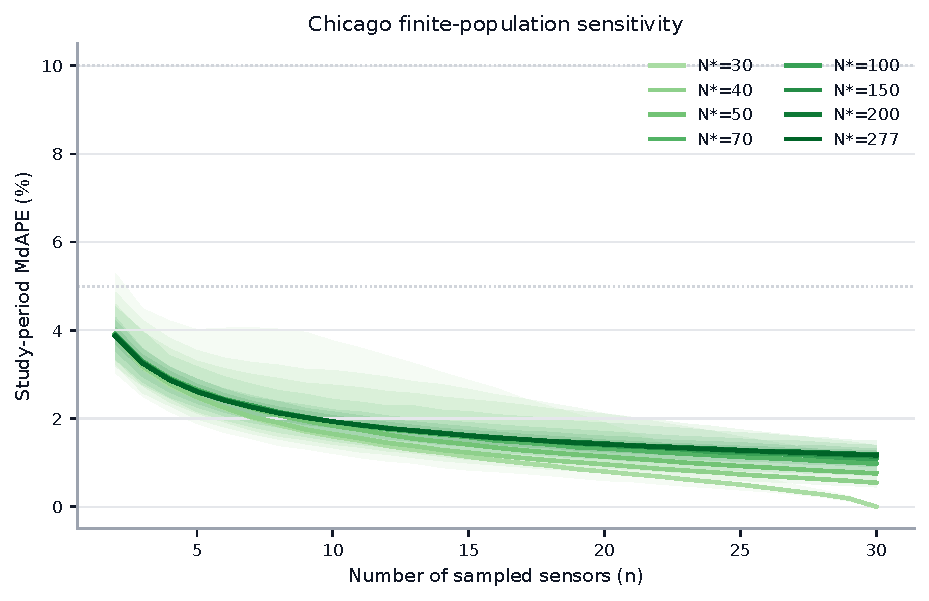
\includegraphics[width=\textwidth]{Plots/Supporting_Information/Figure_SI_17/finite_population_size_sensitivity_chicago.pdf}
 \caption{\city{Chicago} N-sweep.}
 \label{fig:si_finite_pop_chicago}
 \end{subfigure}
 \begin{subfigure}{0.49\textwidth}
 \centering
 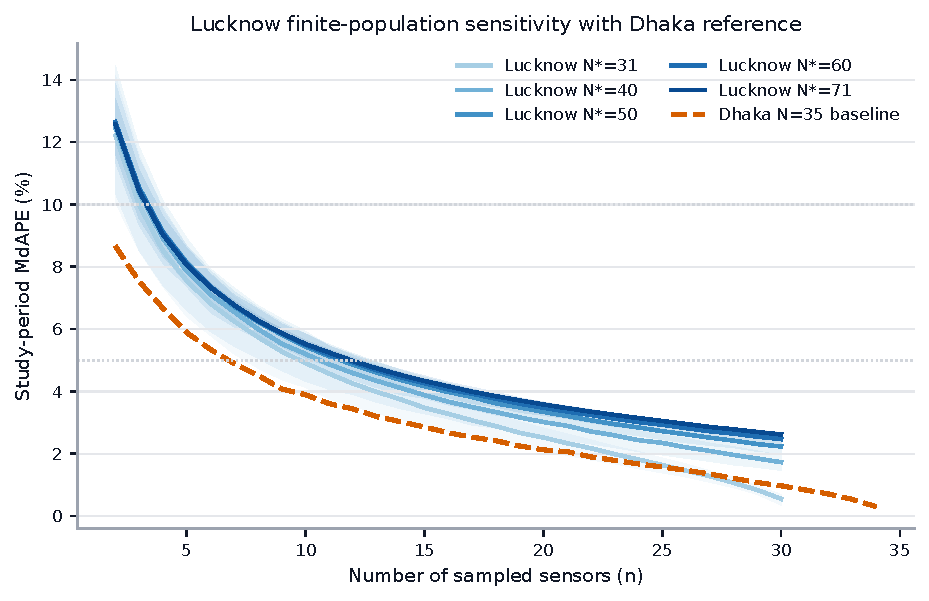
\includegraphics[width=\textwidth]{Plots/Supporting_Information/Figure_SI_17/finite_population_size_sensitivity_lucknow_vs_dhaka.pdf}
 \caption{\city{Lucknow} $N^*=31$ vs.\ \city{Dhaka} $N=35$.}
 \label{fig:si_finite_pop_lucknow_vs_dhaka}
 \end{subfigure}
 \caption{Sensitivity of period MdAPE to the size of the underlying deployed network. (a) Median period MdAPE vs.\ subnetwork size $n$ for \city{Chicago} at $N^* \in \{30, 40, 50, 70, 100, 150, 200, 277\}$, with shaded $5$--$95\%$ across-draw bands; the required $n$ for MdAPE $\le 5\%$ stays at $n=2$ across the entire sweep. (b) \city{Lucknow} downsampled to $N^*=31$ to approximately match \city{Dhaka}'s $N=35$; the \city{Lucknow}-vs-\city{Dhaka} gap persists at matched finite-population size.}
 \label{fig:si_finite_population_sensitivity}
\end{figure}

\subsection{Reference-target sensitivity (dual-reference Monte Carlo)}\label{sec:si_reference_target_sensitivity}

The empirical placement-strategy comparison in Section~\ref{sec:si_placement_empirical} evaluates subnetwork error against the mean of the selected finite population, the standard within-population estimand of SRSWOR. A second, equally interesting estimand is the full-deployed-network mean: the question is whether a small or non-randomly-selected subnetwork can reproduce not only its own internal mean but also the full-deployed-network quantity represented by all available sensors. The two targets are not identical when the selection is non-uniform.

We therefore re-evaluated the same Monte Carlo draws used for the \city{Chicago} selection-strategy comparison against both reference targets: the selected $N^*=50$ mean (within-population estimand) and the full $N=277$ mean (full-deployed-network estimand). Headline numbers are in the released analysis outputs. Period-MdAPE results at $n=10$ are reported in Table~\ref{tab:si_dual_reference}.

\begin{table}[ht]
\centering
\small
\caption{Period MdAPE at $n=10$ against the selected $N^*=50$ mean and against the full \city{Chicago} $N=277$ mean for each \city{Chicago} selection strategy. ``$\Delta$'' is the median of draw-level full-reference MdAPE minus selected-reference MdAPE, so it is not necessarily identical to the difference between the two displayed median columns.}
\label{tab:si_dual_reference}
\begin{tabular}{lrrr}
\toprule
\textbf{Strategy} & vs.\ selected $N^*=50$ & vs.\ full $N=277$ & $\Delta$ \\
\midrule
Random & 1.74\% & 1.91\% & $+0.07$ pp \\
k-means stratified & 1.75\% & 1.84\% & $+0.05$ pp \\
Cluster-concentrated & 1.64\% & 2.14\% & $+0.33$ pp \\
Anti-cluster & 2.26\% & 3.00\% & $+0.76$ pp \\
Spatially balanced & 2.22\% & 2.69\% & $+0.41$ pp \\
Circumferential & 2.10\% & 2.36\% & $+0.36$ pp \\
\bottomrule
\end{tabular}
\end{table}

Two patterns emerge from Table~\ref{tab:si_dual_reference}. First, when the selection is spatially representative (random or k-means stratified), the selected-reference and full-reference targets are essentially the same quantity: the deltas remain small ($0.05$--$0.07$ percentage points). Second, when the selection is clustered or otherwise non-representative (cluster-concentrated, anti-cluster, spatially balanced, circumferential), there is a measurable penalty when the target switches to the full-network mean: the draw-level median deltas range from $0.33$ to $0.76$ percentage points. The cluster-concentrated case is informative: it has the lowest MdAPE against its own selected $N^*=50$ reference because the cluster is internally homogeneous and therefore easy to reproduce, but a $0.33$~pp penalty appears as soon as the target shifts to the full-network mean. This is the empirical version of the cautionary note in the main text that a clustered deployment can reproduce its own mean cheaply while mis-representing the full-deployed-network quantity.

\clearpage

\begin{figure}[H]
 \centering
 \begin{subfigure}{0.72\textwidth}
 \centering
 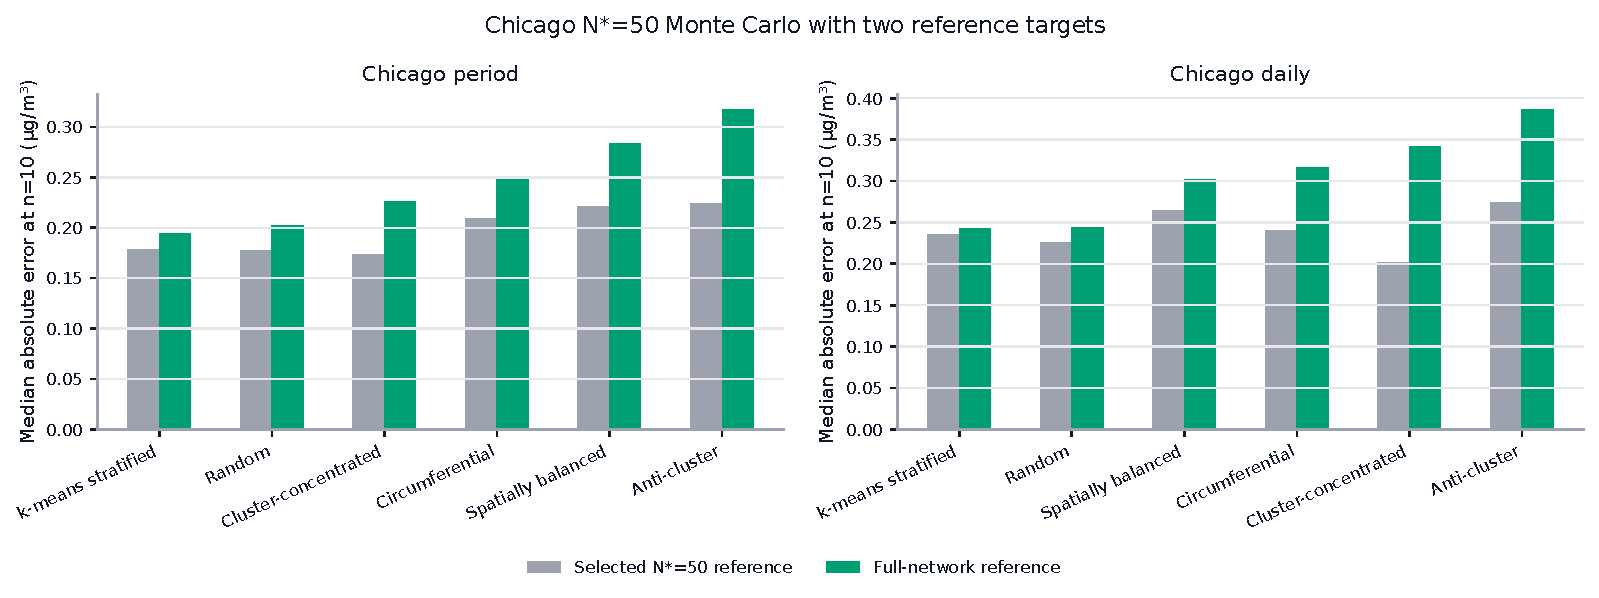
\includegraphics[width=\textwidth]{Plots/Supporting_Information/Figure_SI_18/reference_target_sensitivity_selected_vs_full.pdf}
 \caption{Selected-reference vs.\ full-reference absolute error.}
 \label{fig:si_dual_reference_abs}
 \end{subfigure}
 \vspace{0.05em}
 \begin{subfigure}{0.72\textwidth}
 \centering
 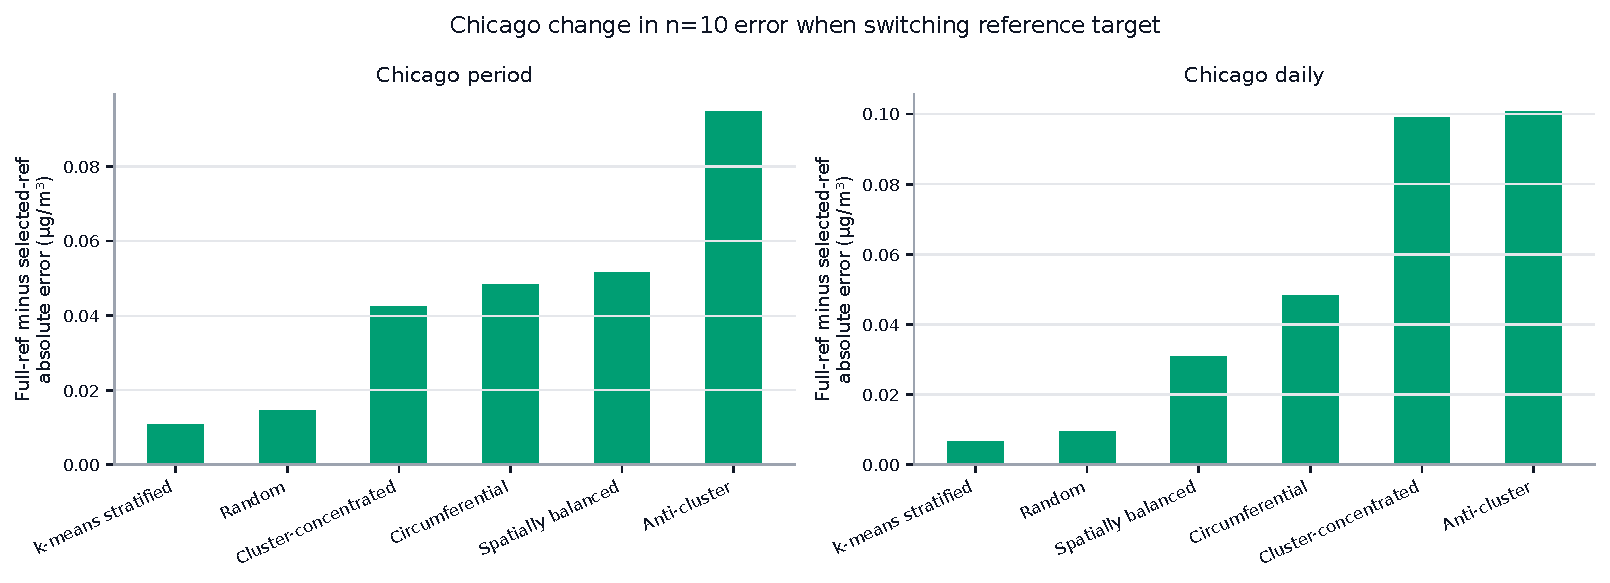
\includegraphics[width=\textwidth]{Plots/Supporting_Information/Figure_SI_18/reference_target_sensitivity_delta.pdf}
 \caption{Full-minus-selected delta by strategy.}
 \label{fig:si_dual_reference_delta}
 \end{subfigure}
 \caption{Reference-target sensitivity at $n=10$, $N^*=50$ in \city{Chicago}. (a) Median daily absolute concentration error against the selected $N^*=50$ mean and against the full \city{Chicago} $N=277$ mean for each selection strategy. (b) The full-minus-selected delta, ordered by strategy. Random and k-means stratified selections (spread well across the network footprint) reproduce both targets essentially equally; cluster-concentrated and anti-cluster selections (deliberately non-representative) pay a visible penalty when the estimand switches from the selected mean to the full-network mean.}
 \label{fig:si_reference_target}
\end{figure}

\subsection{Seed stability of the strategy comparison}\label{sec:si_seed_stability}

We repeated the \city{Chicago} $N^*=50$ strategy comparison under $10$ independent master seeds, with $10$ outer finite-population draws per seed and $B=10{,}000$ inner SRSWOR draws per task. The strategy ordering is qualitatively preserved across seeds. Across-seed median MdAPE-at-$n=10$ values are cluster-concentrated $1.76\%$, k-means stratified $1.77\%$, random $1.81\%$, circumferential $1.97\%$, anti-cluster $2.28\%$, and spatially balanced $2.34\%$, with cluster-concentrated remaining near the low-MdAPE end and spatially balanced or anti-cluster remaining near the high-MdAPE end across seeds. The anti-cluster strategy has the tightest seed band ($5$--$95\%$ width $0.03$~pp), as expected for a fully deterministic selection; spatially balanced and random have the widest bands ($0.56$ and $0.55$~pp, respectively).

\begin{figure}[H]
 \centering
 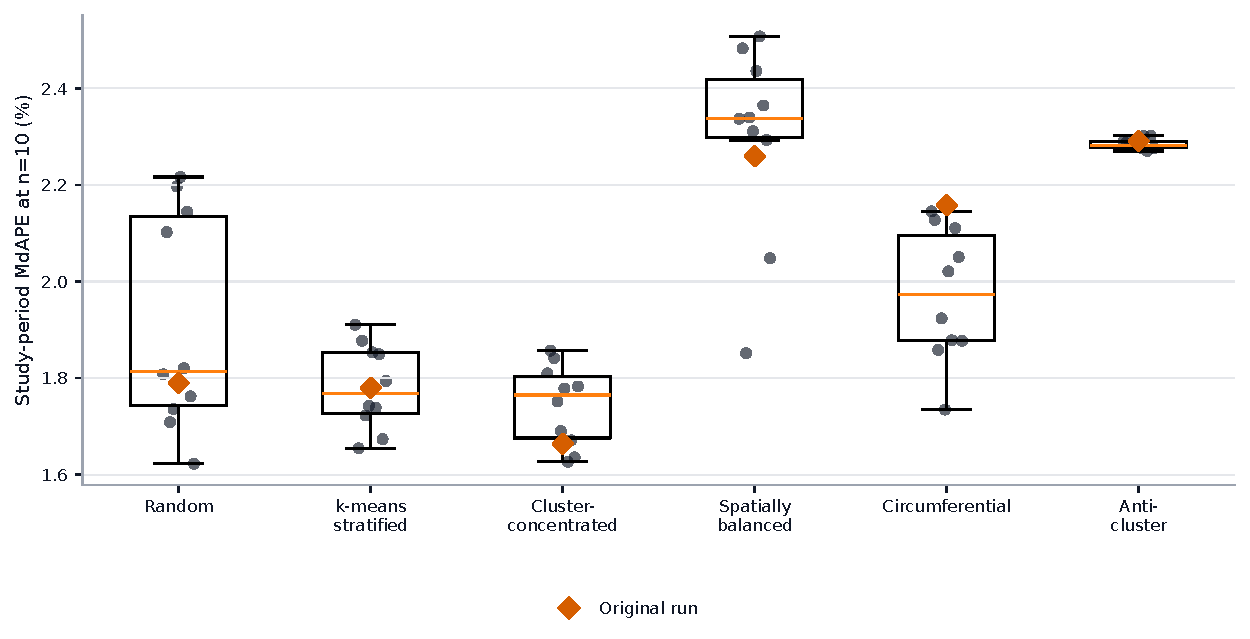
\includegraphics[width=0.78\textwidth]{Plots/Supporting_Information/Figure_SI_19/seed_stability_phase4_strategy_mdape_n10.pdf}
 \caption{Ten-seed stability check for the \city{Chicago} $N^*=50$ selection-strategy comparison. Points show median period MdAPE at $n=10$ for each repeated master seed; diamonds mark the original run. The seed-to-seed spread does not change the qualitative strategy ordering.}
 \label{fig:si_seed_stability}
\end{figure}
